\documentclass[12pt, conference, final, a4paper, onecolumn, compsoc]{IEEEtran}
% Font size onecolumn or twocolumn Use draft for notes or final for no spacing

% Includegraphics
\usepackage{graphicx}
% Coloured code
\usepackage{color}
% Code listings
\usepackage{listings} \lstset{ basicstyle=\small, showstringspaces=false,
  % commentstyle=\itshape\small\color{gray},
  % keywordstyle=\color{cyan}\bfseries, numberstyle=\color{gray}, numbers=left,
  % numbersep=8pt
}
% Bibliography
\usepackage{natbib}
% Figure positions
\usepackage{float}
% Wrapping figures
\usepackage{wrapfig}
% Wrapping URLs
\usepackage[hyphens]{url}
% Changes size of font in captions
\usepackage{caption}
\DeclareCaptionFont{captionfontsize}{\fontsize{12}{14}\selectfont}
\captionsetup{font=captionfontsize}

\begin{document}


\title{Malware Detection within Object Storage} \author{Author: Matthew
  Battagel, Supervisor: Theodoros Spyridopoulos} \markboth{Cardiff University -
  CM3203 - Final Report}{}
\maketitle{}

\subsection*{Acknowledgments - }
% Remove section from TOC TODO TOC: Only showing section
\addtocontents{toc}{\protect\setcounter{tocdepth}{-1}}

I would like to extend my sincere gratitude to my supervisor Theo, my colleague
Harry, friends, family, and Lo for their unwavering support and encouragement
during my project. Their combined expertise and guidance provided were critical
in the shaping and execution of the project. I am truly grateful to all of them
for their contributions.

\bigskip

\begin{abstract}
  Lorem Ipsum
\end{abstract}

\pagebreak

% Problem and background Understanding of the problem and the aims and
% objectives of the project Awareness of the background of the problem

% Detailed analysis of the problem, suitability of approach towards solving the
% problem Solution to the problem Approach and design Solution, implementation
% Use of and justification for appropriate tools/methods

% Evaluation Testing and validation Critical appraisal of results

% Achievement of agreed overall deliverables given in the initial plan for the
% final report (or a justified modification of these) Communication and project
% management skills Written communication skills Project planning, control and
% reflection Interaction and work with the supervisor


% Contents
\tableofcontents{}


\section{Introduction}
\subsection*{Overview}
\paragraph{}
% Data growth and object storage
The exponential growth of data generation has made data storage an increasingly
important aspect for both individuals and organizations alike. Object storage
has emerged as a promising solution due to its ability to store vast amounts of
unstructured data in a cost-effective and scalable manner. Unlike traditional
storage techniques, object storage stores data as objects with related metadata
and unique identifiers, allowing for efficient and cheap storage within buckets.

% TODO Overview: Re-word last part

% Market and competition
One of the most widely used object storage platforms is Amazon S3, which
provides a highly scalable and reliable solution for storing data. However, an
open-source alternative called MinIO has emerged as a promising contender,
providing similar features to Amazon S3 while giving customers greater control
over their data. MinIO is written in Go and is available for free under the
Apache License 3.0 or, for commercial and enterprise purposes, at a reduced cost
compared to Amazon S3 \citep{minio-pricing}. MinIO offers a wide range of
features, including high performance, data replication, encryption and erasure
coding \citep{minio}. Most importantly, MinIO is designed to scale out
horizontally to ensure that it can handle the demands of large-scale
applications.

% Scalability
Scalability is made simple by allowing multiple types of hardware platforms to
work together in separate nodes each with their own compute and storage. This is
extremely attractive for customers who want to utilises their existing hardware
without being tied down to a specific provider. This also applies for customers
looking to migrate their data from Amazon S3 to cheaper solution without
compromising on the high performance, reliability and scalability of the S3
platform.

% Downsides
While MinIO is a great alternative to Amazon S3, it does not offer any form of
malware detection integration. This could put customers off from choosing MinIO
as a viable platform to migrate to from Amazon S3 or leave existing users data
vulnerable to malware attacks. This project aims to address this issue by
integrating a malware detection system into MinIO. An important goal for the is
to negatively impact the scalability or performance as little as possible so
that MinIO is still an effective alternative to Amazon S3.

\subsection*{Motivation} % Why am I trying to add malware detection for object storage?
% TODO Motivation: Can I say about HPE? Or shall I say its for the good of the
% world

Due to the high amount of unstructured data expected to be both written and read
to the object store, there are increased risk of encountering malicious files.
Therefore malware detection within object storage is crucial in modern cloud
storage scenarios. Most popular off-the-shelf object storage platforms, such as
AWS, already have integrated third-party antivirus software, such as ClamAV and
Sophos \citep{amazon-md}, to mitigate security risks. MinIO on the other hand is
vulnerable to malware attacks as it currently does not have any native antivirus
integration. This forces customers who require complete virus protection to
either not use MinIO or to use potentially costly third-party software. As
antivirus scanning is inherently resource intensive, if the software is
integrated incorrectly, it could reduce the ability for the storage solution to
scale horizontally which negates one of the major benefits of object storage.
The purpose of this project is to implement malware detection within MinIO while
being mindful to not impact the scalability or performance of the platform.

\subsection*{Project Aims} % What the project aims to achieve

% TODO Project Aims: This is more about personal goals for the project.

\paragraph{}
From a personal perspective, by completing this project


\section{Background}

% background should be more previous research material etc. Include competition
% and potential software to use e.g. ClamAV, MinIO. Include the first things you
% find when googling the same topic as diss.

% Where to put background info on object storage and malware? Not sure
%

% Insert background material
%

\subsection*{Amazon S3 Malware Detection} % How does amazon do it?
\paragraph{}

As MinIO's largest competitor, this project draws a lot of inspiration from
Amazon S3s integrated malware detection blog page \citep{amazon-md}. The blog
explains Amazons current approach for managing malware detection within their
service. Amazon S3 uses a combination of ClamAV and Sophos as their third-party
scanning engines due to their out-of-the-box nature. Amazon then gives you the
option to use either of these engines or both. The blog goes on to describe the
three main interaction mechanisms that Amazon S3 uses to flag files for
scanning. Firstly, an API endpoint would be provided to handle all uploads. This
forms a queue of uploads which are then scanned before entering the bucket.
Next, event-driven scanning is used keep track of all regular file uploads. The
antivirus will then scan each file after they have been written to the bucket.
Finally, retro-driven scanning is used to scan all existing files within the
bucket. The user then has the flexibility to define what types of files should
be scanned including defining time windows. This blog has given some useful
methodologies of how to keeping track of both incoming and previously scanned
files. Creating a system that can match these methods is important for offering
a matching level of scalability and security within MinIO.

% Talk about standard flow and two bucket flow - useful in designing

% Amazon use stub files

\subsection*{} % How does signature detection work?


\subsection*{} % Best ways of implementing AV into a micro-service?


\subsection*{} % How does ClamAV work? What is clamd

% Malware Artificial Intelligence Object Storage Context

\section{Specification}

The specification for this project is to help guide the project to fulfill the
aims set out in the previous section. The specification is broken down into
three main sections; functional requirements, non-functional requirements and
constraints.

\subsection*{Functional Requirements}
\paragraph{}

Functional requirements are used to define how the solution must work for the
project to be considered a success. This project aims to supply an end-to-end
solution for detecting malware within the MinIO object storage platform. This
goal can be separated into a list of functional requirements:

\begin{itemize}
  \item Provide a way of detecting the latest uploads to the object store.
  \item Record the results of the malware detection within the object store.
  \item Provision for future expansion and ongoing maintenance.
  \item Have a high level of customisability to allow for different use cases.
  \item Allow for efficient and transparent debugging in the event of failure.
  \item Provide the ability to measure various metrics.
  \item Scale alongside MinIO to ensure that it does not bottleneck the object
        store at high loads.
\end{itemize}

% TODO Functional Requirements: End with a sentence?

% TODO Functional Requirements: Say about we need to keep up so that people are
% not waiting and the system does not get behind. Maybe use metrics to show how
% we DO keep up?


\subsection*{Non-Functional Requirements}
\paragraph{}

Non-functional requirements are used to define the quality of the solution that
is required. This project aims to be production ready and therefore the solution
must be held to a high standard. These high standards come in the form of
ambitious targets in which the solution will have to satisfy in order to be
considered production-ready. The non-functional requirements are split into five
categories with metrics to measure their success.

\begin{itemize}
  \item Speed - The solution must be able to keep up with the rate of uploads
        made to MinIO. This can be measured by comparing the time difference
        between uploading a object to MinIO and the object being scanned and
        tagged.
  \item Availability - Over a long period of time the solution must be able to
        handle all requests. This can be measured by comparing the number of
        requests made to the number of requests completed over a large time
        frame.
  \item Capacity - The solution must be able to handle the maximum number of
        simultaneous requests that MinIO can handle. This can be measured by
        monitoring the amount of cache used by the solution under load.
  \item Reliability - 100\% of the files uploaded to MinIO must go through the
        scanning process. The recorded metrics can be used to compare MinIO
        uploads with the number of objects scanned. It is worth noting that
        checking the clean and infected results add to the total sum of scanned
        objects
  \item Usability - Future additions, maintenance and debugging must be as
        simple as possible. This requirement is more subjective and therefore
        explanation of how I have achieved this will be discussed in the
        implementation section.
\end{itemize}

\subsection*{Constraints}
\paragraph{}

The constraints are the limitations that the solution must adhere to. The main
constraint of the project is the strict time limit given to the project. There
are a total of 12 weeks to achieve a production ready product which will greatly
limit the scope of the project. This means accurately prioritising the features
that are most important to the project while also balancing the time spent to
implement them. The second constraint is the limited resources available to the
project.


Another constraint of the project is that all the external software used must be
open source / available for commercial use under license or fee. This is to
ensure that the project is legally viable if the solution was to be used
commercially.

The final constraint is that my own knowledge and experience will increase the
average time taken to implement milestones. This is due to the fact that I will
need to both include time to learn each new technology and also allot excess
time if I incorrectly size a task.

% TODO Constraints: Make sure I mitigate this somewhere

\section{Architecture}

\paragraph{}
Choosing the correct architecture for the project is critical for ensuring that
the solution is scalable, performant and maintainable. Given the specification
above, various potential architectures can be created and evaluated based my own
thoughts and from reading the background material. The best candidate design
will then be chosen based on which candidate design satisfies the most
requirement with as little compromises as possible. Thought will also be given
to which architecture fits within the constraints of the project.

% TODO Architecture: Crop the diagrams to remove the white space

% Post-Write
\subsection*{Candidate Design 1 - Post-Write}
\paragraph{}

The first candidate design makes use of the performance benefits of MinIO by
allowing puts to be initially written to the bucket without being scanned. The
design then uses a event queue compatible with MinIO to keep track of all the
files that have been uploaded. The queue is then used to trigger a scan of the
file once an antivirus is available. The candidate design is shown in figure
\ref{fig:postWriteArch}.

\begin{wrapfigure}{r}{0.45\textwidth}
  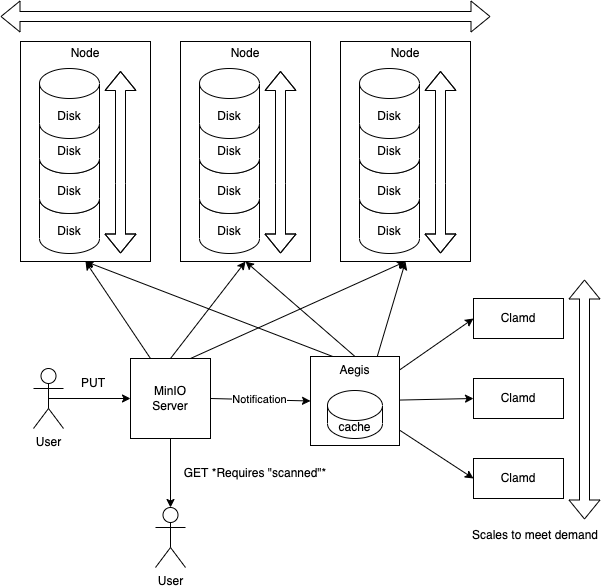
\includegraphics[scale=.4]{diagrams/post-write.png}
  \caption{Post-Write Architecture}
  \label{fig:postWriteArch}
\end{wrapfigure}

This design has many benefits over other potential implementations. Firstly, it
uses the storage provided by MinIO to store all incoming files without having to
manage a separate storage solution. This removes a lot of complexity from the
solution by not having to account for a number of failure conditions that could
occur with a high availability, production ready storage solution. For example,
the solution would not be responsible for handling partial writes, loss of data,
or data corruption. Removing this responsibility allows the solution to focus on
the core functionality of the project, the scanning of files, which is essential
for keeping the project within the time constraints.

Secondly, the design also makes use of the integrated event queue provided by
MinIO. This again removes responsibility from the solution by differing the
scalability and reliability requirements of an event queue to MinIO.

% TODO Candidate Design 1: DO THEY KNOW WHAT AEGIS IS?

Lastly, having Aegis dispatch the files to a scalable number of antivirus
scanners allows the solution to scale to meet the demands of the system. This
meets a key requirement as the solution is expected to have the capacity for a
large number of operations. This method does require the use of a load balancer
to effectively distribute the load across the available antivirus scanners.

The candidate design also has a number of drawbacks. Firstly, the design still
requires a small about of cache to temporarily store the object when it is being
dispatched to the antivirus. Provisioning of this cache has to be large enough
to handle the largest file possible to be uploaded to the object store. In
reality, this cache would be provisioned even larger to allow for the temporary
storage of multiple objects while multiple scans are being performed
asynchronously. In addition, the cache needs to be large enough to ensure that
the system does not become overwhelmed by the number of objects being scanned as
the system scales. This is a minor issue as store capacity is cheap and the
provisioning of the cache easy to scale up. Additionally, a higher priority can
be given to scaling up and out antivirus scanners to ensure that the smallest
number of files are being cached, while bring scanned, at any point.

% TODO Candidate Design 1: Do they know what get/put is? Do they know
% distributed storage topologies?

The second drawback is that, for each event, Aegis makes a get request for the
object to be scanned. This effectively doubles the number of requests made to
the object store. This also means that Aegis must have the ability to get any
file expected to be scanned and therefore must have access to the whole storage
network. The impact of this drawback is mitigated as the solution is expected to
be deployed on the same network as the object store which should reduce the
latency of each request made by Aegis. However, this still leaves MinIO to
handle twice as many requests with the performance loss being noticed mainly on
more distributed storage topologies.

Thirdly, the candidate design only allows for a single Aegis instance to
dispatch all incoming objects to available scanners. This is a potential
bottleneck for the system as this instance could become overwhelmed by the
number of requests it is receiving. This is a minor issue as the dispatching of
objects to scanners is not as performance intensive as other areas of the
solution, such as the actual scanning, and therefore it is not expected to be a
major bottleneck.

Lastly, any object uploaded to the store will have a certain period of time
where it remains unchecked. In this time, the user could potentially download an
unscanned object or the object could cause harm to the store before it is
detected. Although the handling of infected objects is out of scope, in an
actual implementation of the solution, the user could be made unable to download
unscanned objects until they have been scanned.

% TODO Candidate Design 1: AWS does this with S3 events 'standard flow'

\subsection*{Candidate Design 2 - Upload Queue}
\paragraph{}

% TODO Candidate Design 2: More explanation here?
This candidate design created a wrapper around MinIO that the user interacts
with instead of MinIO. This means that all puts go through Aegis before being
uploaded to the object store. The candidate design is shown in figure
\ref{fig:uploadQueueArch}.

\begin{wrapfigure}{r}{0.45\textwidth}
  \centering 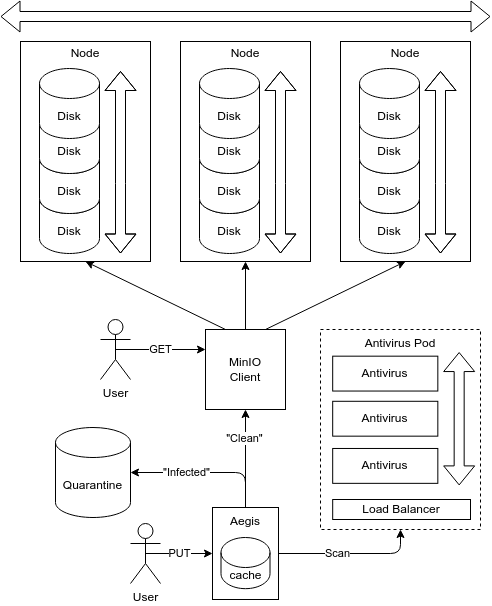
\includegraphics[scale=.4]{diagrams/upload-queue.png}
  \caption{Upload Queue Architecture}
  \label{fig:uploadQueueArch}
\end{wrapfigure}

The main benefit of this design is that the user interacts only with Aegis when
uploading files. This means that all incoming files can be stored within a
temporary storage before ever entering the object store. This offers the best
protection against malicious files as the user cannot ever download an unscanned
or infected file as it is never uploaded to the object store. Infected files can
then either be deleted or moved to a separate quarantine store for analysis.

This candidate designs main advantage also comes with a major drawback. This
design requires Aegis to handle the full throughput of all the puts to the
system. Aegis then has the full responsibility of being available to all puts
and, in a failure scenario, to handle the recovery of the system. Additionally,
the cache provisioned must be large enough to handle the largest files at
maximum throughput with extra room for unexpected delays. This negatively
affects the scope of the project by requiring the solution to prioritise
features that are already covered by MinIO.

% TODO Candidate Design 2: Cover mitigation

% TODO Candidate Design 2: is this already covered?
Because MinIO is dependent on Aegis to handle the puts, MinIO must wait to be
passed incoming objects sequentially after Aegis has finished processing the
previous object. This removes the potential for aggregate performance where

% TODO Candidate Design 2: Talk about how AWS uses this method 'Two Bucket
% System Flow'

\subsection*{Candidate Design 3 - Write Interception}
\paragraph{}

% TODO Candidate Design 3: Edit diagram to show quarantine?

Candidate Design three is very similar to the second candidate design, however,
instead of wrapping outside the MinIO service, it intercepts the writes from the
client before objects are written to the object store. With this interception,
Aegis can scan the object and decide whether to allow the object to be written
to the store or to quarantine the object. The candidate design is shown in
figure \ref{fig:writeInterceptArch}.

\begin{wrapfigure}{r}{0.4\textwidth}
  \centering 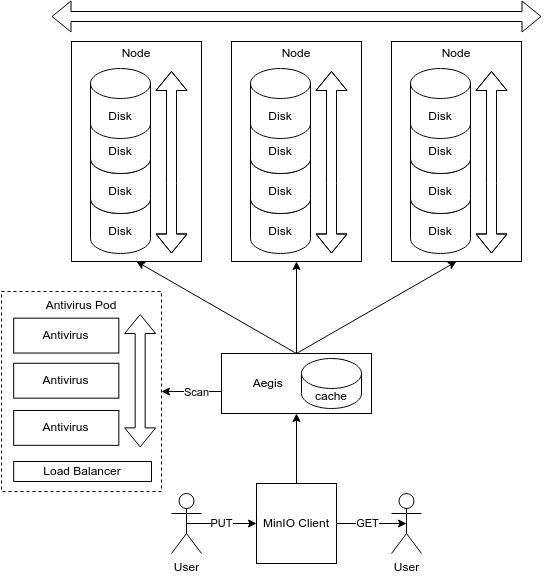
\includegraphics[scale=.3]{diagrams/write-intercept.png}
  \caption{Write Interception Architecture}
  \label{fig:writeInterceptArch}
\end{wrapfigure}

This candidate design has similar benefits as the second candidate design. It
offers the most protection against malicious files by never allowing either
unscanned or infected objects to be stored in the object store. However, it also
has similar drawbacks. This is because Aegis is still in sequence with MinIO
meaning that for optimal throughput, Aegis would need to match the performance
of MinIO.

Similar to the upload queue candidate design, this design also requires Aegis to
have a large cache to handle the largest files at maximum throughput. This cache
must also be large enough to handle the number of objects being put by MinIO
into the store. This issue cannot be mitigated without the risk of compromising
performance at increased loads.

However, this design does have an advantage over the second candidate design as
there is less responsibility placed on Aegis to be as failure tolerant. MinIO is
still directly responsible for accepting objects into the store and therefore is
still responsible for the recovery of the system in a failure scenario. This
allows the scope to focus on more related features to malware scanning.

% TODO Candidate Design 3: Encrypted???

\subsection*{Candidate Design 4 - Per Node}
\paragraph{}

% TODO Candidate Design 4: More?
The final candidate design distributes Aegis onto each node in the object store.
This means that each node has a local instance of Aegis that is responsible for
scanning objects before they are written to the store. The candidate design is
shown in figure \ref{fig:perNodeArch}.

\begin{wrapfigure}{r}{0.5\textwidth}
  \centering 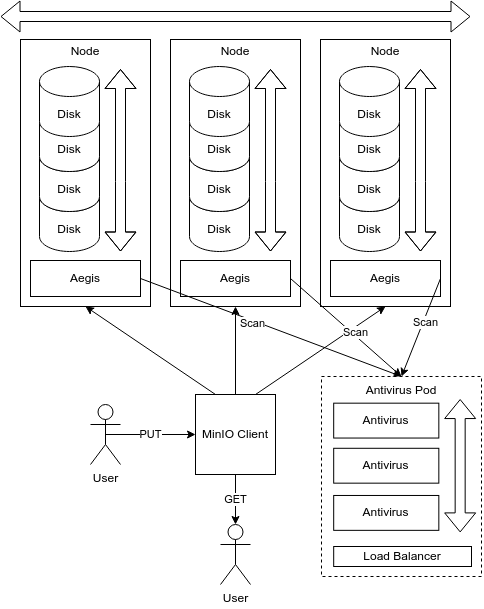
\includegraphics[scale=.3]{diagrams/per-node.png}
  \caption{Antivirus per Node Architecture}
  \label{fig:perNodeArch}
\end{wrapfigure}

This candidate design makes use of the distributed nature of MinIO to match the
demand when scaling out the system. As more nodes are added, more Aegis
instances are added to handle the increased scanning demand. This removes the
need for having a cache repository as Aegis already has access to the files that
need scanning. By removing this single point of failure, in theory, the system
only relies on the antivirus pod to be able to scale out on its own.

Independent scaling of the antivirus pod allow for efficient usage of available
hardware. A simple load based auto-scaler can be used to scale the number of
pods based on the current load. This allows for the system to flexible scale
with the demand of the system and to reduce usage of valuable resources, such as
power. There is also the opportunity to use intelligent scaling techniques to
predict the load on the system and prematurely scale the system to meet the
demand. For example, to scale the number of pods depending on the time of day or
the day of the week.

% TODO Candidate Design 4: Explain MinIO terms
The major drawback of this candidate design is that it replies on the ability to
scan whole files by only using data on a single node. In actual implementations,
MinIO makes use of erasure coding to add increased redundancy to the store
\citep{minio-erasure}. Erasure coding splits objects into multiple parts known
as blocks, and then calculates corresponding parity blocks. These data and
parity blocks are then distributed among all nodes in the system allowing for
on-the-fly data recovery even with the loss of multiple drives or nodes . This
means that the Aegis instance on each node only has access to the part available
on their node and therefore will not be able to reconstruct the whole file for
scanning. This makes this candidate design unsuitable for MinIO as it erasure
coding is one of its key features.


\subsection*{Selected Candidate Design}

Given the above evaluations of each candidate design, design one best meets the
requirements and constraints of the project. It makes the most use of the
existing features that MinIO provides in order to handle failure scenarios and
to scale out. This also means that this design has less critical responsibility
and will better fit the scope constraints allowing for more time to be spent on
supplementary features, such as testing, logging, and metric collection. Because
of this, the produced solution will be closer to production-ready than the other
candidate designs.

This candidate design keeps the user in control by giving them the ability to
store unscanned files / known malware without wasting resources on a scan.
Protection can be added per bucket therefore a user could have a known malware
bucket and a clean bucket within the same object store. This allows for the
system to be more flexible and to be able to handle more use cases. Candidate
Designs two and three would not be as able to handle this use case as they both
scan all objects before they are written to the store.

The size of the cache required is smaller than all other candidate designs as it
only needs to store the objects actively being scanned. This is in opposition to
upload queue and write interception candidate designs as they have to be
prepared to handle the full demand placed on the store. This makes candidate
design one the most lightweight of all the candidate designs which should lead
to a smaller resource footprint.

% TODO Selected Candidate Design: This is a bad ending :(
Overall, implementing candidate design one is the best option to create a
lightweight yet secure and scalable solution.

\section{Implementation}

% TODO Implementation: What does the final product look like?

\subsection*{Service Selection and Creation} % How I tested each service

% TODO Implementation: Why did I choose to start all the services separately?

Before I started to code the solution, I needed to research, create, configure
and most importantly understand each external service that I would be using. Up
to this point I know what types of services I would need to create, but I did
not know what specific services I would be using. This section will go through
the process of how I chose each service and then initially configured them to
form a bare-bones proof of concept.

\subsubsection*{Object Store - MinIO}
\paragraph{}

The object store is the only service that I did not need to research or compare
as it is already the subject of this project. However; I did need to create and
configure a local instance of MinIO for development. MinIO itself is available
from many sources, including Docker, Homebrew, and the MinIO website. I chose to
use Homebrew, a MacOS package manager, as it is the easiest to install and
update. I then used the MinIO documentation to create a local instance of MinIO
where I can access the web client on \url{http://localhost:9000}. From this I
could create buckets, upload objects to the store and get more familiar with
MinIO's features.

% TODO Object Store: Include images

MinIO has integrated the ability to send notifications to event queues depending
on what operation is performed on the store. This makes it quick and easy to set
up a locally running instance of an event queue to read messages sent by MinIO.
MinIO offers wide support for many different event queues, such as Kafka,
Webhook, Redis, PostgreSQL, and many more.

\subsubsection*{Event Queue}
\paragraph{}

Kafka is a popular and well-supported event queue that is used in many different
industries. It offers many features that make it a good choice for this project,
such as high-throughput, low latency and open-source. Kafka is also available
from both Docker and Homebrew make it easy to install and run locally. Most
modern event queues offer similar high throughput and low latency, but Kafka is
lighter in resource usage than other queues, such as RabbitMQ
\citep{kafka-rabbitmq}. This is beneficial as it will be easier to implement and
not over use resources when it has a simple use case.

Kafka has a dependency on Zookeeper, which is a distributed coordination
service. Zookeeper must be installed as a separate service but is available from
the same sources as Kafka. Kafka can be run in Kafka Raft mode (KRaft) which
will eventually replace Zookeeper, but as of writing KRaft has not been fully
adopted yet \citep{kafka-raft}.

With Kafka and Zookeeper setup, I use Kafka's command line interface (CLI) to
start the service and create a topic. I then use the MinIO documentation to
configure MinIO to send all put notifications to the Kafka topic. I can then use
the Kafka CLI to read messages from the topic and see the messages sent by
MinIO. This proves that the event queue is working and that MinIO is sending
messages to it whenever I perform a put operation. An example Kafka message is
available in the appendix in listing \ref{kafka-notif}.

% TODO Event Queue: Reference TODO Object Store: Include images?

\subsubsection*{Antivirus}
\paragraph{}

The antivirus we choose has to meet a list of requirements for it to be suitable
for use in this project. Firstly, it must be able to be scaled with the solution
in order to keep up with the demand placed on the system. Secondly, it must have
a CLI that our program can interact with in order to scan files. Finally, it
must be free or as cheap as possible to make it viable for commercial use. This
narrows down the available options to a few contenders.

Sophos is a popular antivirus that is used by many businesses and is available
for free for personal use, however; is it paid % TODO Antivirus: Sophos

ClamAV however is completely free and open-source. It comes with a scalable and
multi-threaded daemon which can be accessed via CLI for high-performance and
on-demand file scanning. \citep{clamav}. It is capable of scanning many
different file types, including archives and mail files. Build-in is freshclam,
a tool for automatically updating the virus database definitions. The virus
database itself is also open-source and is updated regularly by the open source
community. ClamAV has a docker image and is available from Homebrew.

I have chosen to use ClamAV as it is totally free for commercial use,
open-source and has a CLI that can be used to scan files. It is also very well
documented and has a large community of users. Sophos
% TODO Antivirus: Sophos too expensive

ClamAV comes with a daemon, clamd, that can be run in the background and can be
accessed via a CLI using clamdscan, the clamd client. A configuration file is
needed to point clamdscan to the IP address that the daemon is running. In this
case it is running locally on port 3310. Performing the clamdscan command and
providing a file will scan the file and return the result. An example of this is
available in the appendix in listing \ref{clamd-scan}.

% TODO Object Store: Include images?

\subsubsection*{Metric Collection}
\paragraph{}

As the project is expected to be as production-ready as possible, a system for
collecting metrics is needed. This will allow the system to monitor its activity
for easier maintenance and debugging. A few different options are available for
metric collection, such as Prometheus, InfluxDB, and Graphite. Each of these

% TODO Metric Collection: Reference why we need metrics

% TODO Metric Collection: Complete comparison

From this comparison, I chose to use Prometheus as it is open-source, uses a
pull model with the option for a push gateway and it does not require a
distributed system to run, unlike InfluxDB. Prometheus is available from both
Docker and Homebrew.

Prometheus is currently unusable as I am not sending it any metrics to collect.
I can still launch the Prometheus server and access the web interface on port
9090. In the meantime I can use the Prometheus documentation to create a
configuration file defining the port and endpoint I expect to be exposing
metrics to, in this case port 2112 and /metrics.

% TODO Metric Collection: Shall I reference Prometheus docs?
s
% TODO Object Store: Include images?

\subsubsection*{Audit Log Store}
\paragraph{}

Production-ready software should have a way to store logs for auditing and
analysis purposes. This is a relatively simple requirement as a central database
can be used due to the expected low amount of data needing to be written. The
purpose of the audit log is to store information about the scans performed by
the system with information such as, time and result of the scan as well as the
antivirus used. This gives the system a way to look back at previous scans which
could help with debugging and maintenance.

There are many different options for a database to store the audit logs, such as
PostgreSQL, MySQL, MongoDB, and many more. PostgreSQL remains the most versatile
out of these options as it is a relational database and can be used for many
different purposes. As the use case is simple, keeping to a single database
service is the best option for maintainability and usability. PostgreSQL is also
available from both Docker and Homebrew.

% TODO Audit Log Store: Compare some more databases?

Like Prometheus, PostgreSQL is currently unusable as I am not sending it any
data to store. However, I can still launch the PostgreSQL server and access the
database via PostgreSQL shell prompt (psql). I can create a database and a user
for the database to use. This database can then be exposed to port 5432 on the
localhost ready for Aegis to use.

% TODO Audit Log Store: Reference why we need metrics TODO Object Store: Include
% images?

\subsubsection*{Data Visualisation}
\paragraph{}


% TODO Data Visualisation: Why we need data visualisation
Grafana

% TODO Data Visualisation: Compare other data visualisation tools - prometheus

Compare

% TODO Initial Service: Docker?? Or include that in each service
Docker

% TODO Object Store: Include images?


\subsection*{Aegis Design and Creation}
\paragraph{}

Now all of the dependencies have been downloaded, initialised and configured,
Aegis can now be coded to interact with them.


The most common language to use for micro-service based projects is GoLang. Go
is a compiled language that is statically typed and high concurrency support.
This makes it a perfect fit for this project to ensure that the system is as
performant as possible. MinIO is also written in Go should allow for easier
integration. Go has certain standards and guidelines for clean architecture that
should be followed to ensure high usability and efficiency.

\subsubsection*{Project Structure}
\paragraph{}

In Go you should the separate the code into different packages, where each
package represents a distinct function of the system. This allows for easier
maintenance and debugging in the future. These packages are then grouped into
different directories depending on their intended scope and function. There are
three main directories that are used in GoLang projects, cmd, pkg and internal.
The cmd directory is used to store the main.go file which manages the workflow
and is the entry point of the program. The pkg directory is used to store all of
the packages that are intended to be used by external applications, in this case
our other services. The internal directory is used to store all of the packages
that are intended to be used by the application itself. This is where the
packages in the pkg directory will be consumed to perform the Aegis' core
actions as follows:

\begin{itemize}
  \item Listen for PUT events on the event queue
  \item Read the message from the event queue and extract the bucket and object
        path
  \item GET the object from the object store and store in cache
  \item Initiate a scan on the object using the antivirus software
  \item Collect the result of the scan and add tags to the object
  \item Collect metrics throughout the process
  \item Store the result of the scan in the audit log
  \item Expose metrics to Prometheus
\end{itemize}

From these requirements, the internal design of Aegis can be planned. We can
visualise this plan using a class diagram. It is worth noting that Go itself
does not have classed but instead uses structs which can be used to achieve the
same effect. This plan is shown in figure \ref{fig:aegisPlan}.

\begin{wrapfigure}{r}{0.4\textwidth}
  \centering 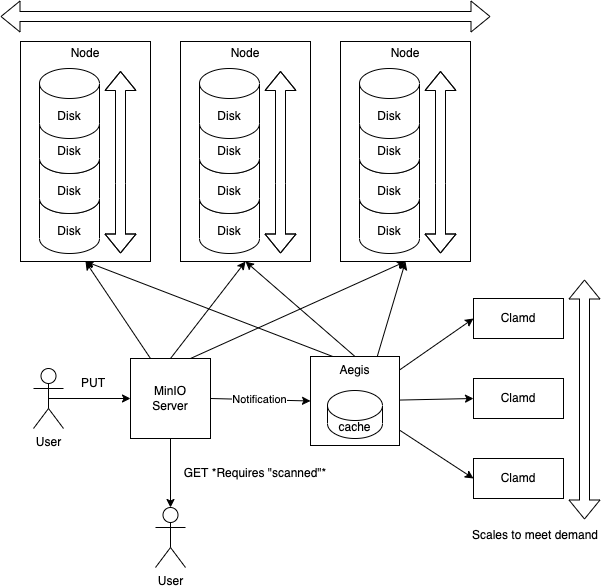
\includegraphics[scale=.3]{diagrams/aegis-class-diagram.png}
  \caption{Plan of Aegis' Internal Packages}
  \label{fig:aegisPlan}
  \bigskip \centering 
\includegraphics[scale=.3]{diagrams/aegis-file-struct.png}
  \caption{Aegis' Initial File Structure}
  \label{fig:aegisFileStruct}
\end{wrapfigure}

% TODO Aegis: Class diagram

From this diagram a file structure can be created inline with Go standards. Go
comes with a CLI tool used to initialise a new go module, which is a collection
of packages that are intended to be used together. This tool will create a go
mod file which is used to define the module and its dependencies. This tool will
also create a go sum file which is used to store the hashes of the dependencies
to ensure that the same version is used across all environments. Now go commands
can be used to install go dependencies and then download them to a local vendor
folder for use in building. Building the project is also done with the go CLI.
All binaries are stored within the build folder. The initial project structure
is shown by the figure \ref{fig:aegisFileStruct}.

\subsubsection*{Version Control}
\paragraph{}
I decided that due to the size of this project, that version control would be
necessary to ensure that the project is maintainable and that there is always a
backup available. I chose to use Git in combination with GitHub as I am very
familiar with the platform and it is free to use. I used the Git CLI to
initialise a new repository within the root directory of the go module. In
addition, I created a git ignore file to ensure that the vendor and build
folders are not uploaded.

In order to retain usability, throughout the project I will be committing to the
remote GitHub repository after each significant change to the project while
including relevant commit messages. This will make it easier to track changes
for debugging and maintenance purposes.

\subsubsection*{Structured Logging}
\paragraph{}

Structured logging is a method of logging that allows for easier parsing of the
log messages by adding structure to the message. This is done by adding key
value pairs containing relevant information to the log message. This enables for
easier filtering and searching of the logs. This is especially useful when using
a log aggregation tool such as Humio.

Go has many external modules that can handle this type of logging including Zap
by Uber. Zap is a very fast and efficient logging library that can be configured
to change the level of logging output, such as for info or debug useful for
production or development respectively \citep{zap-repo}. Zap also has the
ability to change between structured and unstructured logging depending on the
use case. Structured logging comes with the drawback of being less human
readable than unstructured logging and therefore Zap offers the ability to
change between the two \citep{zap-repo}.

% TODO Structure Logging: Humio Ref, Structured logging ref. Zap ref

As Zap is an external module, it must be added as a dependency and all code
contained in the pkg folder. A package called logger is created to encapsulate
all logging functionality. This package contains two go files, one for
interacting with the Zap and one for defining the structure of the log commands
inside of an interface. In Go, it is idiomatic to keep the interface as close to
the implementation as possible. Keeping the interface in the same package as the
implementation allows for easier mocking of the package when testing. This
package goes against this by containing the interface within the repository
because multiple packages will need to use the same interface when interacting
with them. This reduces code duplication as we don't have to define the
interface in each package that uses it, which in this case would be every
package. The code is shown in figure \ref{fig:logger-code} and the interface is
shown in figure \ref{fig:logger-interface}.

% TODO Structure Logging: Include code extracts TODO Structure Logging: Example
% of using the interface?

\subsubsection*{Configuration}
\paragraph{}

As Aegis is a micro-service, it is important that it is configurable to allow
for easy deployment to different environments. This is done by using a
configuration file in tandem with Viper, a Go module that can read in the
configuration file.

This configuration file contains all of the values that are likely to change
between environments. This includes values such as the endpoints, ports and
credentials of external services, logging options and database names. This
configuration file will be a dotenv file which is a key value store of
environment variables. This is beneficial as Viper has the ability automatically
override the config file with environment variables if the same key is found.
This allows for easier configuration of the application when it is built locally
or deployed in a kubernetes cluster. This gives the user the ability to tailor
the deployment to their needs or existing implementation.

Much like the logger package, the configuration package contains two go files. A
repository file that defines the interface and a config file that contains the
Viper configuration.

% TODO Configuration: Figure of dotenv and explain mapstructure

% TODO Configuration: Viper repository reference

Adding both the configuration and structured logging as the first packages
reduces the need for refactoring in the future. No hard coded values are needed
for initial development as all values can be stored in the configuration file
from the start.

\subsubsection*{Testing}
\paragraph{}

% TODO Testing: Explain Mockery

\subsubsection*{Makefile}
\paragraph{}

A Makefile is a file that contains a set of instructions that can be run from
the command line. These instructions are used to automate processes such as
building, testing and deploying. Through the project, longer workflows will be
automated and put into the Makefile to reduce the amount of time spent on
running commands. Makefiles also simplify the usage of program by users by
encapsulating complex commands into an explicit action the user can understand.
Makefile commands can also be used by the Dockerfile when building the
application in a container.

% The Makefile is available for viewing in the repository

% TODO Makefile: Link to GitHub


\subsection*{External Package Integration}
\paragraph{}

With the dependency services still running, the next step is to integrate them
into the Aegis application using Go. This is done by creating a new package for
each of the services within the pkg folder. Each package will contain a go file
for each of the services that will later be consumed by Aegis' internal
workflow.

One significant advantage of separating external services from internal
implementation is that it allows for a higher level of abstraction from the
services used. This abstraction provides flexibility in the use of multiple
external services that fulfill the same purpose, such as multiple antivirus
scanners. The creation of external packages allows for the use of a single
internal implementation for all of these services. This reduces the need for
extensive changes in the future, making the application more maintainable and
scalable.
% TODO SOMEWHERE: Explain that capitals mean exported in Go

\subsubsection*{MinIO}
\paragraph{}

The initial external service to be incorporated is MinIO. The MinIO package
manages interactions with the MinIO service. For this project, the required
operations include getting, putting, and removing objects, as well as getting
and putting tags. MinIO provides a Go Software Development Kit (SDK) that
already supports these operations in Go \citep{minio-go-repo}. The SDK
simplifies the complexities of making requests and offers straightforward
methods for operations such as putting and getting, as well as accessing type
definitions like tags.

Once the MinIO SDK is imported, a new MinIO client object is generated to
communicate with the MinIO service. The \texttt{CreateMinio} function accepts
essential connection parameters, such as a context, an endpoint, access and
secret keys, and an SSL usage flag, and initializes the MinIO client using the
\texttt{minio.New} function. This client object is then incorporated into a
custom \texttt{Minio} struct, along with a logger. Various methods are
implemented for the Minio struct to execute different object storage operations:

\begin{itemize}
  \item \texttt{GetObject}: Retrieves an object from a specified bucket and
        returns its data as a byte slice.
  \item \texttt{PutObject}: Takes in a byte stream and uploads it to a specified
        bucket with a specified object name.
  \item \texttt{RemoveObject}: Removes a specified object from a specified
        bucket.
  \item \texttt{GetObjectTagging}: Fetches the tags associated with an object
        and returns them as a map of key-value pairs.
  \item \texttt{PutObjectTagging}: Replaces the existing tags of an object with
        a new set of tags provided as a map of key-value pairs.
  \item \texttt{AddObjectTagging}: Adds new tags to an object by first fetching
        the existing tags, updating them with the new key-value pairs, and then
        setting the updated tags back to the object. Necessary for not
        overriding existing object tags that may exist.
\end{itemize}

All of these methods take in a context which is used in the shutdown process to
close the connection to the MinIO service. This context is passed in during the
creation of the MinIO struct so that all methods have access.

\subsubsection*{Kafka}
\paragraph{}

The next external service to be integrated is Kafka. The Kafka package will
handle the interactions with the Kafka service. For this project, the operations
needed are to consume messages from a specified topic. Kafka provides a Go
library, \textit{kafka-go}, which simplifies the consumption of messages in a Go
application \citep{kafka-go-repo}.

The package imports necessary dependencies and creates a custom
\texttt{KafkaConsumer} struct, which embeds a \texttt{kafka.Reader} object and a
logger. The \texttt{CreateKafkaConsumer} function initializes a new
\texttt{KafkaConsumer} instance by taking connection parameters such as the list
of brokers, the topic to be consumed, a group ID, and a maximum number of bytes
per message.

\begin{itemize}
  \item \texttt{ReadMessage}: Uses the Kafka library to halt until a message is
        received from the specified topic. It then decodes it using the
        \texttt{decodeMessage} function, and returns the bucket name and object
        key.
  \item \texttt{decodeMessage}: Decodes a Kafka message by unmarshalling its
        JSON payload and extracting the bucket name and object key. If the
        message event is \textit{s3:ObjectCreated:PutTagging}, it returns empty
        strings, as this event does not require processing.
\end{itemize}

During the shutdown process, the \texttt{ReadMessage} function is halted by
closing the context passed in. This closes the connection to the Kafka service
and therefore stops the reading of any new Kafka messages, leaving unprocessed
messages in the event queue.

\subsubsection*{ClamAV}
\paragraph{}

ClamAV is another external service to be integrated into the project. The
primary operation needed for this project is scanning a file and returning the
scan results. The ClamAV daemon can be interacted with through the command-line
interface (CLI) using the \texttt{clamdscan} command \citep{clamav-repo}.

Initially, a \texttt{ClamAVScanner} struct is created, embedding a logger. The
\texttt{CreateClamAV} function initializes a new \texttt{ClamAVScanner}
instance. Methods for the \texttt{ClamAVScanner} struct are implemented to
perform various file scanning operations:

\begin{itemize}
  \item \texttt{ScanFile}: Accepts a file path as an argument and scans the file
        using the built-in Go exec library to run the \texttt{clamdscan} command
        with the \texttt{--config} flag set to use a custom configuration file
        located at \texttt{clamav.conf}. The exec library enables the execution
        of external commands, providing the ability to interact with the ClamAV
        antivirus daemon. A process attribute is added, which starts the process
        in a different process group than the main execution. This approach aids
        in achieving a graceful shutdown later on, as calling a system interrupt
        terminates the entire process group \citep{process-groups}. As a result,
        \texttt{ScanFile} can continue executing after the shutdown, ensuring
        that no scans are interrupted. The method returns false if the file is
        clean, true if infected, and the type of malware detected. If any errors
        occur during the execution, it returns true (infected) along with an
        error message, ensuring that the worst-case scenario is assumed when it
        comes to security.
  \item \texttt{findVirusType}: Takes the output from the \texttt{clamdscan}
        command, extracts the virus type using regular expressions, and returns
        it as a string.
  \item \texttt{GetName}: Returns the name of the antivirus engine, in this
        case, "clamav". The name must be accessed through a method, as ClamAV
        will implement an interface that does not have access to any attributes.
\end{itemize}

The internal scanner package can now use the ClamAV package as one of the
antivirus engines to scan files it receives.

\subsubsection*{Prometheus}
\paragraph{}

The Prometheus package is in charge of creating and managing an HTTP server that
exports metrics from Aegis. It does this by providing a plaintext response
containing the metrics in the Prometheus exposition format. The exposed endpoint
is then used by the Prometheus server to collect metrics from Aegis.

\begin{itemize}
  \item \texttt{CreatePrometheusServer}: Initializes a new Prometheus exporter
        by setting up a new HTTP server with the specified endpoint and path.
        The Prometheus handler, provided by the \texttt{promhttp.Handler()}
        function from the Prometheus Go client library, is linked to the given
        path, which serves the plaintext. Read and write timeouts for the HTTP
        server are established using constants since these values are not
        expected to be configurable.
  \item \texttt{Start}: Initiates the Prometheus server by calling the
        \texttt{ListenAndServe()} method on the HTTP server. An example of the
        generated plaintext output can be found in the appendix at listing
        \ref{example-exposed-metrics}.
  \item \texttt{Stop}: Handles the graceful shutdown of the Prometheus server by
        invoking the \texttt{Shutdown} method to close the HTTP server.
\end{itemize}
% TODO Prometheus: Maybe include diagram? TODO Prometheus: Is implement used
% correctly?

\subsubsection*{PostgreSQL}
\paragraph{}

The package imports necessary dependencies and creates a custom
\texttt{PostgresqlDB} struct, which embeds a \texttt{pgxpool.Pool} object and a
logger. The \texttt{CreatePostgresqlDB} function initializes a new
\texttt{PostgresqlDB} instance by taking connection parameters such as the user,
password, endpoint, and database name. It also returns a \texttt{CloseFunc}
function to close the connection when needed.

\begin{itemize}
  \item \texttt{CreatePostgresqlDB}: Is responsible for establishing a
        connection to the PostgreSQL database and returning a
        \texttt{PostgresqlDB} instance. The function takes in connection
        parameters such as the user, password, endpoint and database name.
        Additionally, it returns a \texttt{CloseFunc} function to facilitate a
        graceful shutdown of the connection pool when necessary. Instead of
        connecting straight to the database, the function uses a connection pool
        to manage connections. This allows multiple concurrent clients to
        perform operations on the database without having to wait for other
        clients to finish their transactions. In this case, when multiple files
        are being scanned at the same time and the results are being saved to
        the database, the connection pool ensures that a database connection is
        always available.
  \item \texttt{CreateTable}: Uses the connection pool to create a new table
        with the specified name if it does not exist. The table schema includes
        columns for ID, ObjectKey, BucketName, Result, Antivirus, Timestamp, and
        VirusType. The SQL query used to execute this operation is available in
        the appendix at listing \ref{create-table-query}.
  \item \texttt{Insert}: Uses the connection pool to insert a record into the
        specified table with values for ObjectKey, BucketName, Result,
        Antivirus, Timestamp, and VirusType. The SQL query used to insert is
        available in the appendix at listing \ref{insert-query}.
\end{itemize}

The PostgreSQL instance is provided with a context to close the connection to
the database when the application is shutting down.

\subsection*{Aegis' Internal Workflow}
\paragraph{}
% TODO Aegis' Internal Workflow: Describe what internal means

s
% TODO Aegis' Internal Workflow: Explain what channels are?

\subsubsection*{Metrics and Collectors}
\paragraph{}

The internal metrics collection comprises two primary components: the metric
manager and various metric collectors specific to each package. The metric
manager is responsible for managing interactions with Prometheus, which includes
executing the \texttt{Start} and \texttt{Stop} methods for handling the starting
and graceful shutdown of Prometheus respectively.

Each package contains a metric collector in a file named \texttt{metrics.go}.
These collectors define the available metrics that can be collected and exported
by the respective packages. The \texttt{promauto} library facilitates the
creation of a global registry when the metric manager is initialized. This
registry is accessed by all metric collectors to record the metrics they collect
and is also utilized by the Prometheus exporter for publishing these metrics.

\subsubsection*{Object}
\paragraph{}

The object package presents the \texttt{Object} struct as the internal
representation of an object within the object store. It includes all methods and
attributes related to an object, such as the object key and bucket name.
Operations involving an object are performed within the object instance itself.

Since the object represents a concrete entity, there is no need for an interface
when using it. This design choice allows the object to have attributes that can
be accessed directly, without the need for getter functions.

The \texttt{CreateObject} function enables the creation of a new \texttt{Object}
instance, given a specified object key and bucket name.

The \texttt{SetCachePath} method defines the cache path for an object by
concatenating the cache path, bucket name, and object key, separated by slashes.
This method is called when an update to the cache path is needed.

The \texttt{SaveByteStreamToFile} method stores an object's byte stream in a
file. First, it checks if the path attribute is empty since, by default, no path
is provided. It returns an error if this is the case, as other types of scanners
may not always require this information to perform a scan. Next, it ensures that
the file's parent directory exists, creating it if necessary. Lastly, the method
writes the byte stream to the file using Go's built-in IO writer.

The \texttt{RemoveFileFromCache} method is responsible for deleting an object
file from the cache. It tries to remove the file specified by the object's path
attribute. If the removal is unsuccessful, it logs an error message and returns
the error.
% TODO Object: Why object KEY?

\subsubsection*{Events Manager}
\paragraph{}
The events package includes the event manager, which is responsible for reading
messages from the event queue and forwarding scan requests to the scanner. The
\texttt{Kafka} interface provides methods for reading messages from the Kafka
queue and closing the connection. The \texttt{EventsManager} struct consists of
four fields: a \texttt{logger}, a \texttt{kafka} instance for interacting with
Kafka, a \texttt{scanChan} channel to forward scan requests and an
\texttt{eventsCollector} for gathering metrics.

% TODO Events Manager: Explain switch? Concrete types

The \texttt{CreateEventsManager} function creates a new \texttt{EventsManager}
instance, accepting the necessary arguments. The \texttt{Start} method of the
\texttt{EventsManager} takes in a context and then enters a loop that uses a
switch statement to first check if the context has been canceled. If it has, it
closes the \texttt{scanChan} channel, closes the Kafka connection and returns.
Otherwise, it invokes the \texttt{ReadMessage} method of the \texttt{kafka}
instance to read a message from the Kafka queue. Upon confirming that there is
no error and the message is not nil, it increments the \texttt{eventsCollector}
counter and creates a new \texttt{object.Object} instance with the received
bucket name and object key. It then forwards the object to the \texttt{scanChan}
channel for scanning.

Since the event manager runs within a goroutine, if an error occurs, it sends
the error to the provided \texttt{errChan} channel.

\subsubsection*{Object Store}
\paragraph{}
In the object store package, several structs and interfaces are defined to
handle object storage operations. The \texttt{Minio} interface contains the
abstract object store operations, such as; get, put and remove objects, as well
as get and put object tags. These are also reflected by the
\texttt{ObjectStoreCollector} in the form of metric counters that track the
number of each operation performed.

Once the object store is created by the \texttt{CreateObjectStore} function, it
can be used by the rest of the application to perform object storage operations.
In addition to the standard object storage operations, two more operations are
added to the object store: \texttt{MoveObject} and \texttt{AddObjectTagging}.
These both combine multiple standard operations into one as follows:

\begin{itemize}
  \item \texttt{MoveObject}: Retrieves an object from the source bucket, puts it
  into the destination bucket, and removes it from the source bucket.
  \item \texttt{AddObjectTagging}: Retrieves the object tags from the source
  bucket, adds the new tags to the existing ones, and puts the combined object
  tags onto the object.
\end{itemize}

\subsubsection*{Object Scanner}
\paragraph{}
The scanner package provides the functionality for multiple workflows when it
comes to scanning an object. In this instance, an object scanners downloads from
the object store, performs a scan with its antivirus engines, and then passes
the result to a cleaner which will execute the cleanup policy. Having the
ability to use multiple types of scanners allows for flexibility in the system
as in the future, the workflow for scanning an object might change. For example,
if one of the antivirus engines could require the hash of the file. In this
case, another scanner called \texttt{HashScanner} could be created to handle
this alternate workflow. For this project, the \texttt{ObjectScanner} will be
the only type of scanner implemented.

The \texttt{CreateObjectScanner} function creates a new \texttt{ObjectScanner}
instance with the following arguments:

\medskip
\begin{itemize}
  \item \texttt{logger}: A logger instance for logging messages.
  \item \texttt{objectStore}: An object store instance for downloading objects.
  \item \texttt{antiviruses}: An array of antivirus instances for scanning
        objects.
  \item \texttt{cleaner}: A cleaner instance for cleaning up objects.
  \item \texttt{auditLogger}: An audit logger instance for logging scan results.
  \item \texttt{scanCollector}: A scan collector instance for collecting
        metrics.
  \item Various configuration values, such as, \texttt{removeAfterScan},
        \texttt{datetimeFormat}, and \texttt{cachePath}.
\end{itemize}

All instances passed to the \texttt{CreateObjectScanner} function are interfaced
to both allow for future mocking and to allow for other abstract implementations
of the interfaces.

% TODO Object Scanner: Assume the worst mentality explain

The \texttt{ScanObject} method handles the workflow for downloading and scanning
an object. It takes in an \texttt{object.Object} instance, which it fetches from
the object store, and an \texttt{errChan} for returning errors. It then sets the
object cache path by calling \texttt{SetCachePath} on the object. With this set,
the scanner can perform a \texttt{GetObject} on the object store to retrieve the
byte stream of the object and call \texttt{SaveByteStreamToCache} with the byte
stream to save it to the cache.

The scanner can now perform a scan on the object by calling \texttt{Scan}, with
the cache location, on every antivirus engine. If any of the antivirus engines
detect the object as infected, then using the assume the worst mentality, the
file is deemed infected. The object is then passed to the cleaner to execute the
cleanup policy. During this execution various metrics are being collected by the
\texttt{scanCollector} about the scan, such as, the number of clean or infected
files, total files scanned and total errors encountered. In addition audit logs
are also generated by the \texttt{auditLogger} for each scan by each antivirus,
recording the object key, bucket name, antivirus name, scan result, timestamp
and if infected, the virus type.

After performing the scan and dealing with the results, if the
\texttt{removeAfterScan} flag is set to true, the object is removed from the
cache after scanning.

The \texttt{ObjectScanner} is will be run within a goroutine, if an error is
encountered during the scan, it will be sent to the provided \texttt{errChan}.

\subsubsection*{Cleanup Policies}
\paragraph{}

% TODO Cleanup Policies: Read again

As mentioned in the previous section, the \texttt{ObjectScanner} passes the
object to the cleaner to execute the cleanup policy. The cleaner package defines
how to react given a clean or infected result from the antivirus engines.
Multiple policies are available in the \texttt{config.env} file to give the user
flexibility in how they want to deal with infected objects. These policies
include:

\begin{itemize}
  \item \texttt{Tag}: Adds a tag to the object in the object store based on the
        scan result.
  \item \texttt{Remove}: Removes the object from the object store if it is
        deemed infected
  \item \texttt{Quarantine}: Moves the object to a quarantine bucket if it is
        deemed infected.
\end{itemize}

In \texttt{CreateCleaner} function, a new \texttt{Cleaner} instance is created
with a logger, object store, metrics and audit loggers, and various
configuration parameters such as the cleanup policy and quarantine bucket.

The \texttt{Cleanup} method is called by the \texttt{ObjectScanner} where is
passes the object after it has been scanned. This method uses a switch
statement, shown in figure \ref{cleaner-switch}, to determine which policy to
implement and executes the appropriate cleanup method. If no policy is
specified, the switch statement has a default cause of logging that it will do
nothing, in the case that the user only wants the audit logs. However with a
given cleanup policy, the corresponding cleanup method is called. Each of these
use the object store and object store to perform the cleanup.

\begin{figure}[H]
\begin{lstlisting}[language=Go]
    switch c.cleanupPolicy {
    case "tag":
      err = c.TagInfected(object, result, scanTime)
    case "remove":
      err = c.RemoveInfected(object, result, scanTime)
    case "quarantine":
      err = c.QuarantineInfected(object, result, scanTime)
    default:
      c.logger.Warnln("No cleanup policy found")
    }
\end{lstlisting}
  \caption{Cleanup policy switch statement}
  \label{fig:cleaner-switch}
\end{figure}

\subsubsection*{Dispatcher}
\paragraph{}
% TODO Dispatcher: Is implement correct?
%
% TODO Dispatcher: Explain go keyword

The \texttt{dispatcher} package is responsible for managing the scanning of
objects using multiple scanners concurrently. It defines a \texttt{Scanner}
interface with a single method, \texttt{ScanObject}, that will be implemented by
one of the available scanners. The \texttt{Dispatcher} struct contains three
fields: a \texttt{logger} for logging messages, a \texttt{scanChan} channel for
receiving object scan requests, with a \texttt{scanners} slice to hold the
available scanners.

The \texttt{CreateDispatcher} initialises a new \texttt{Dispatcher} instance
with the required fields. The \texttt{Start} method enters into a loop where it
ranges over the \texttt{scanChan} channel. If the channel is empty, the loop
will block until a new object is sent through the channel. If the channel has an
object, the dispatcher will spawn a new goroutine to handle the scan. However,
if the channel is closed, the loop will continue to process all objects in the
channel and then exit \citep{go-channel-ranges}. This is because when channels
are closed, no more values can be sent to them, but the values that have already
been sent can still be received \citep{go-closing-channels}. This is shown in
the provided dispatcher loop code in figure \ref{fig:dispatcher-loop}.

\begin{figure}[H]
\begin{lstlisting}[language=Go]
func (d *Dispatcher) Start(errChan chan error, done chan struct{}) {
	var wg sync.WaitGroup

	for request := range d.scanChan {
		for _, scanner := range d.scanners {
			wg.Add(1)
			go func(req *object.Object, sc Scanner) {
				defer wg.Done()
				sc.ScanObject(req, errChan)
			}(request, scanner)
		}
	}
	wg.Wait()
	done <- struct{}{} //Send empty done message
}
\end{lstlisting}
  \caption{Dispatcher loop}
  \label{fig:dispatcher-loop}
\end{figure}

When the program receives a termination signal, there should be no loss of
information about incoming scan requests. This is a security risk as it could
lead to objects not being scanned. To prevent this, the dispatcher uses a
\texttt{sync.WaitGroup} to wait for all goroutines to finish before exiting the
program. This is done by calling \texttt{wg.Add(1)} before starting a new
anonymous goroutine to increment an active goroutine counter, and using
\texttt{defer wg.Done()} when the goroutine has finished to decrement the
counter. The \texttt{wg.Wait()} call will block until the counter is zero,
meaning all goroutines will have finishes processing \citep{go-waitgroups}. This
ensures that all scans that are currently being processed since
\texttt{scanChan} was close will be completed before the program exits.

% TODO Dispatcher: Explain defer

\subsubsection*{Main}
\paragraph{}


The main package orchestrates the top-level workflow that Aegis executes
throughout its operation. The entry point of the program is the \texttt{main}
function, which performs one task - calling the \texttt{run} function and
exiting the program based on its return value. This design choice enhances
extensibility and testability since alternate workflows can be implemented while
maintaining a single entry point. Furthermore, the \texttt{run} function can be
tested without running the entire program \citep{go-tiny-abstraction}. The
\texttt{run} function serves as a abstraction from \texttt{main}, as it
encompasses Aegis' main workflow.

The \texttt{run} function is divided into three distinct sections:
initialization and configuration, the main loop, and cleanup. The initialization
and configuration section is responsible for initializing all the components
Aegis requires and configuring them with the values provided by the
configuration package.

\medskip
\begin{itemize}
  \item The configuration is loaded from \texttt{config.env}, and the logger is
        created. An initial context is also created and passed to everything
        that requires it, apart from the event system.
  \item The metric manager and various metric collectors are created, with the
        metric manager taking in the Prometheus exporter.
  \item The audit logger is implemented by the PostgreSQL database.
  \item The object store is implemented by the Minio client.
  \item The event system is implemented by the Kafka consumer with the
        \texttt{scanChan} passed in as well.
  \item The scanning workflow is created. This includes creating the antivirus
        engines, in this case ClamAV, creating the cleaner with the configured
        policy and passing both of them to the scanners, namely the object
        scanner. The scanners are then passed to the dispatcher alongside the
        \texttt{scanChan}.
\end{itemize}
\bigskip

% TODO Main: Parameter tree?

% ---- Main loop -----

The main loop is the continuous execution of the goroutines that handle Aegis'
asynchronous operations. These are the event manager, dispatcher, and metric
manager. The goroutines are started using the \texttt{go} keyword, which spawns
a new goroutine to execute the functions in a separate thread.

An additional context is created and parsed into the \texttt{Start} method of
the \texttt{eventManager}. Multiple channels are then created to handle errors,
shutdown command, and the shutdown complete with \texttt{errChan},
\texttt{shutdownChan} and \texttt{done} respectively. The \texttt{Start} methods
of the \texttt{eventManager}, \texttt{dispatcher} and \texttt{metricManager} are
called to begin the main workflow of the program.

An error channel (\texttt{errChan}) is created to handle errors generated by the
event manager and metric manager goroutines.


% ---- Shutdown -----

Finally, the shutdown section ensures a smooth termination when the program
receives an interrupt signal or encounters errors from the goroutines. The
shutdown sequence is vital as it allows Aegis to maintain the progress of
processed objects when receiving messages, enabling it to resume scanning
objects from where it left off upon restart. The shutdown sequence unfolds as
follows:

When an interrupt signal or an error from any goroutine is received, Aegis
starts its graceful shutdown sequence. A select statement is used to wait for a
message from either the \texttt{errChan} or \texttt{shutdownChan} channels. If
any of these channels receive a message, a message or error is logged, and the
shutdown sequence begins by canceling the context passed to the event manager.
This action halts the event manager from consuming messages from the Kafka
consumer and subsequently closes the \texttt{scanChan} channel. As a result,
incoming notifications remain in the Kafka queue and can be consumed by Aegis
upon restart leading to no scans lost.

The code then waits for the \texttt{done} channel to send a message, signaling
that the goroutines have completed processing the remaining objects in the
\texttt{scanChan} channel. Once this process is finished, the program stops the
Prometheus metric exporter and exits with a status code of 0, indicating a
successful operation.

% TODO Graceful Shutdown: Explain select??

\subsection*{Testing}

\subsubsection*{Mocking}
\paragraph{}

\subsubsection*{Unit Tests}
\paragraph{}

\subsection*{Kubernetes Deployment}
\paragraph{}



\subsubsection*{Docker}
\paragraph{}

\subsubsection*{Aegis Containerisation}
\paragraph{}

\subsubsection*{Kubernetes}
\paragraph{}

\subsubsection*{Helm}
\paragraph{}

\subsubsection*{K3d}
\paragraph{}

\section{Results and Evaluation}
% Evaluate against specification Compare to MinIO Find figures like average scan
% Compare local vs cluster
\subsection*{}

\section{Product Issues / Future work} % What you would do next time
\subsection*{}

\section{Conclusions}
\subsection*{}

\section{Reflection on Learning} % Fuck knows
\subsection*{}

\section{Appendix}
% TODO Appendix: Add figures and tables to appendix
%
%
%
\lstinputlisting[caption={Example Kafka Notification}, label=kafka-notif,
numbers=left]{assets/example-notif.json}

\bigskip \lstinputlisting[caption={Example Kafka Notification},
label=clamd-scan]{assets/example-clamd-scan.txt}

\bigskip \lstinputlisting[caption={Example Exposed Metrics},
label=example-exposed-metrics]{assets/example-exposed-metrics.txt}

\bigskip \lstinputlisting[language=SQL, caption={Create Table SQL Query},
label=create-table-query]{assets/create-table-query.txt}

\bigskip \lstinputlisting[language=SQL, caption={Insert into Table SQL Query},
label=insert-query]{assets/insert-query.txt} \bigskip

\bibliographystyle{cardiff} \bibliography{references}

\end{document}

% TEMPLATED
% \begin{figure}[!ht]
%   \centering \includegraphics[scale=.55]{assets/extracred}
%   \caption{Bouncing and pitching motion as a function of time}
%   \label{fig:bounceAndPitch}
% \end{figure}

% \begin{table}[!ht]
%   \begin{center}
%     \caption{Calculated values}
%     \label{tab:calculated}
%     \begin{tabular}{|c|c|}
%       \hline
%     \end{tabular}
%   \end{center}
% \end{table}

% Appendix \onecolumn \textwidth=456pt \paperwidth=577pt \hoffset=-30pt
% \newpage
% \newpage
% \clearpage


% \pagestyle{headings}
% \section{Appendix A}
% \centering Heading \footnotesize

% \normalsize

% \csvautolongtable{assets/vibProj.csv}
%
